\documentclass[12pt,a4paper]{report}

\usepackage{amsmath}
\usepackage{amssymb}
\usepackage{siunitx}
\usepackage{graphicx}
\usepackage{caption}
\usepackage{subcaption}
\usepackage{cite}
\usepackage{algorithm}
\usepackage{algorithmicx}
\usepackage{algpseudocode}
\usepackage{algpseudocodex}
\usepackage{tikz}
\usepackage{tikz-feynman}
\usepackage[a4paper, margin=2.5cm]{geometry}
\usepackage[colorlinks=true, linkcolor=blue, citecolor=blue, urlcolor=blue]{hyperref}

\usetikzlibrary{positioning}

\captionsetup{font=footnotesize}

\begin{document}

\begin{titlepage}
  \centering
  \vspace*{2cm}
  {\LARGE\bfseries A Lorentz covariant model of string fragmentation \par}
  \vspace{1.5cm}
  \Large Jade Abidi \par
  \vspace{0.5cm}
  \large Student ID: 31461964 \par
  \vspace{0.5cm}
  {\large A thesis submitted for the degree of \bfseries{Bachelor of Science (Honours)}} \par
  \vspace{0.5cm}
  \large November 2025 \par
  \vspace{0.5cm}
  \vfill
  \large School of Physics and Astronomy \\ Monash University \par
  \vspace{0.5cm}
  \large Supervisor: Peter Skands \par
  \vfill
\end{titlepage}

\pagebreak

\begin{abstract}
Monte Carlo event generators are extensively used to simulate high-energy particle-collision events. For analytically intractable aspects, they rely on phenomenological models. The so-called Lund model describes the non-perturbative hadronisation process as the fragmentation of a classical string with constant tension. Lorentz covariance then implies the self-similarity of this fragmentation process along the string. The current formulaion of the Lund model, used in the PYTHIA generator, violates this property in terms of both kinematic distributions and hadronic chemistry. We introduce an additional tunable parameter and a new algorithm for string fragmentation that improve or resolve these issues, albeit with some limitations.
\end{abstract}

\pagebreak

\tableofcontents

\chapter{Introduction}
The field of particle physics investigates the most fundamental particles and interactions in nature. It naturally evolved from nuclear and atomic physics in the early 20th century as technological and scientific knowledge allowed scientists to probe matter at higher energies and smaller length scales \cite{ParticleDataGroup:2024cfk,Gross:2022hyw}. The physical theory underpinning particle physics developed out of quantum field theory, culminating in the Standard Model of particle physics which was formalised in the 1980s. The Standard Model unifies three of the four fundamental forces of nature (electromagnetism, the weak force, and the strong force) into a single theory, and predicted the existence of the Higgs boson well before its historic discovery at the Large Hadron Collider (LHC) in 2012 \cite{Schwartz:2014sze,ATLAS:2012yve,CMS:2012qbp}.

The interactions investigated in particle-physics experiments occur at high energies, with low probabilities. Particle colliders, such as the LHC, are designed specifically to enable such experiments by accelerating charged particles, usually electrons or protons (and their antiparticles), to speeds up to 99.99999\% of the speed of light. Most modern particle colliders are circular, and use high voltages and strong magnetic fields to accelerate particles and keep them within a thin beamline. The particle beams are then made to collide millions of times every second at interaction points, around which bespoke detector systems collect data on the final state \cite{ParticleDataGroup:2024cfk,Ellis:1996mzs,Evans:2008zzb}.

For comparison against this data, it is very useful to be able to generate ensembles of large numbers of events based on physical models and assumptions. Because the physics involved is so complex and often lacks an analytic solution, Monte Carlo event generators such as PYTHIA provide a way to sample the phase space efficiently \cite{ParticleDataGroup:2024cfk, Bierlich:2022pfr, Buckley:2011ms, Skands:2012ts}. Powerful factorisation theorems allow for the various processes that occur at different energy scales to be modelled independently of each other, which greatly simplifies the problem \cite{Collins:1981uw, Skands:2012ts}. The focus of this project is the process of hadronisation, in which partons (quarks and gluons) form hadronic bound states. This occurs at momentum transfer scales below the confinement energy of $\Lambda_\text{QCD} \sim \qty{0.2}{\giga\electronvolt}$ \cite{Skands:2012ts}.

Due to asymptotic freedom, the coupling constant of the strong force becomes very large for momentum transfers in this range \cite{Gross:1973ju,Politzer:1974fr}, and therefore the physics of hadronisation cannot be calculated perturbatively. Non-perturbative quantum chromodynamics has not yet been analytically solved, and numerical methods such as lattice QCD have limitations that render them inapplicable to hadronisation \cite{Salam:2010zt}. Instead, PYTHIA uses the Lund string model as a description of hadronisation, which is a phenomenological theory (and is not derivable from first principles) \cite{Bierlich:2022pfr,Andersson:1983ia}.

In the Lund string model, the strong field between a quark and antiquark is modelled as a string with constant tension $\kappa \sim \qty{0.9}{\giga\electronvolt}$ per femtometre, as measured in lattice QCD simulations \cite{Bali:1992ab,Skands:2012ts}. At separation distances of $\gtrsim \qty{1}{\femto\meter}$, there is enough potential energy stored in the string for it to ``break'', forming a new quark-antiquark pair. This leaves two quark-antiquark string subsystems, which proceed to break in the same manner as the original system, giving rise to a recursive self-similar process resulting in a set of outgoing bound states of quarks \cite{Andersson:1983ia,Andersson:1997xwk,Bierlich:2022pfr,Skands:2012ts}.

This self-similarity of the fragmentation process along the string is one of the most fundamental properties of the Lund string model. The string breaks are all spacelike separated and hence cannot causally influence each other, and the tension along the string is constant and invariant under longitudinal boosts. It therefore follows that, away from the endpoints of the string, all fragmentation observables (like the number or species of hadrons produced from a region of the string) must be invariant under Lorentz boosts (or equivalently, rapidity translations) along the string axis. This means that distributions such as hadron density per unit rapidity should be flat except for endpoint effects (denoted the ``rapidity plateau''). It also implies that, if considered iteratively, the process by which each string subsystem is fragmented must be scale invariant \cite{Andersson:1983ia,Andersson:1997xwk,Bierlich:2022pfr}.

((TODO: Rewrite this and next paragraph to be more clear about what finalTwo is, what it does, and its importance)). Despite the importance of the Lorentz covariance of string fragmentation in the Lund model, current simulations in PYTHIA reveal that this property is quite badly broken. Since the release of PYTHIA 8.0, the rapidty plateau has exhibited a significant dip in the central region. Initial investigations revealed this to be a consequence of the hadronisation algorithm used in PYTHIA, where the final two hadrons have kinematics forced by energy-momentum conservation and the mass-shell relation. In the Monash tune of PYTHIA 8.3, the rapidity spacing between these final two hadrons is larger than the typical rapidity spacing. This, combined with the non-uniformity of location of the joining step along the string, gives rise to this central rapidity dip. Furthermore, the \texttt{finalTwo} procedure that generates these hadrons fails about 50\% of the time, introducing bias that skews the species makeup of these final two hadrons.

PYTHIA offers three tunable parameters that adjust the behaviour of this procedure --- \texttt{stopMass}, \texttt{stopNewFlav}, and \texttt{stopSmear}. Prior to this project, it was believed that these parameters could be tuned to give a flat rapidity plateau, and would not need to be retuned when other fragmentation parameters change \cite{Bierlich:2022pfr,Sjostrand:2006za}. This is not the case for the Monash tune, where it is impossible to achieve a flat plateau with these parameters without significantly worsening the failure rate of \texttt{finalTwo}.

In this thesis, chapter \hyperref[chap:background]{2} provides a review of the theoretical background of quantum chromodynamics, PYTHIA, and the Lund string model. In chapter \hyperref[chap:fragmentation]{3}, the current behaviour of the PYTHIA hadronisation algorithm is analysed in more detail, and the various problems are described and explained. In chapter \hyperref[chap:tuning]{4}, the tuning of the \texttt{finalTwo} parameters is discussed. An additional tunable parameter \texttt{revertFinalBreak} is presented which provides an additional dimension of parameter space and allows for a flatter rapidity plateau to be obtained without as much of an impact on the failure rate. Finally, in chapter \hyperref[chap:accordion]{5}, an alternative algorithm for hadronisation in PYTHIA is developed, called the accordion join, which achieves an approximately flat rapidity plateau for any tune, and fails more than a hundred times less frequently.

\chapter{QCD, the Lund Model, and PYTHIA}
\label{chap:background}
\section{Quantum Chromodynamics and Collider Physics}
Before introducing PYTHIA and the Lund string model, we first provide an overview of the theoretical models and experimental techniques used in particle physics, with a focus on quantum chromodynamics.

The field of particle physics developed out of the study of atomic and nuclear physics in the early 20th century. Experiments like the discovery of the nucleus in 1911 \cite{Rutherford:1911zz} or the neutron in 1932 \cite{Chadwick:1932wcf} paved the way for the development of more advanced technologies such as particle accelerators and colliders. The high centre-of-mass energies reached in these experiments allowed for the discovery of a slew of particles in the 1950s and 1960s, dubbed the ``particle zoo'' \cite{Gross:2022hyw}. Alongside these experiments, the theoretical success of quantum mechanics inspired the quantisation of the electromagnetic field in the original formulation of quantum field theory (QFT) and quantum electrodynamics (QED) by Dirac, who notably predicted the existence of antimatter a number of years before its discovery \cite{Dirac:1928hu,Anderson:1932zz}. QED was later unified with a description of the weak force (responsible for phenomena like beta decay) into electroweak theory, a Yang-Mills gauge theory consisting of a local $\text{U}(1) \times \text{SU}(2)$ gauge symmetry \cite{ParticleDataGroup:2024cfk,Thomson:2013zua}.

\begin{figure}
  \centering
  \setkeys{Gin}{width=\linewidth}
  \begin{minipage}[t]{0.49\textwidth}
    \centering
    \includegraphics[width=0.7\linewidth]{figures/eightfold-way.png}
    \caption{A visual depiction of the pseudoscalar mesons in the Eightfold Way, which form an octet and a singlet in $\text{SU}(3)$ flavour space\cite{Neeman:1961jhl,Gell-Mann:1962yej}. The horizontal axis represents $I_3$, an isospin component, and the vertical axis represents $Y$, the hypercharge, both of which are quantum numbers arising from the $\text{SU}(3)$ flavour symmetry. Figure taken from \cite{Thomson:2013zua}.}
    \label{fig:eightfold-way}
  \end{minipage}
  \hfill
  \begin{minipage}[t]{0.49\textwidth}
    \centering
    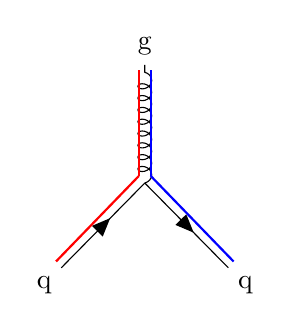
\begin{tikzpicture}
      \begin{feynman}
        \vertex (a);
        \vertex [above=of a] (g) {g};
        \vertex [below left=of a] (q1) {q};
        \vertex [below right=of a] (q2) {q};
        
        \diagram* {
          (q1) -- [fermion] (a) -- [fermion] (q2),
          (a) -- [gluon] (g)
        };

        \draw[red, thick] ($(q1) + 0.15*(1cm,2cm)$) -- ($(a) + 0.15*(-0.5cm,0.6cm)$);
        \draw[blue, thick] ($(q2) + 0.15*(-1cm,2cm)$) -- ($(a) + 0.15*(0.5cm,0.6cm)$);
        \draw[red, thick] ($(a) + 0.15*(-0.5cm,0.6cm)$) -- ($(g) + 0.15*(-0.5cm,-2cm)$);
        \draw[blue, thick] ($(a) + 0.15*(0.5cm,0.6cm)$) -- ($(g) + 0.15*(0.5cm,-2cm)$);
      \end{feynman}
    \end{tikzpicture}
    \caption{An illustration of a $qqg$ vertex in QCD, showing the colour flow. The incoming and outgoing quarks have one colour, while the gluon has two (a colour and anticolour).}
    \label{fig:qqg-vertex}
  \end{minipage}
\end{figure}

At the same time, quantum chromodynamics (QCD) emerged, describing the variety of particles discovered in the ``particle zoo'' as composed of more fundamental subatomic particles --- quarks and gluons. Initial models like the Eightfold Way classified these various strongly interacting particles as hadrons emerging from a $\text{SU}(3)$ flavour symmetry between three quark flavours \cite{Neeman:1961jhl,Gell-Mann:1962yej}, as shown in Figure \ref{fig:eightfold-way}. These flavours were later denoted the up (u), down (d), and strange (s) quarks, and three more (charm, beauty, and top) were eventually found. Hadrons were classified into two groups --- mesons, which are bosonic bound states consisting of a quark and an antiquark, and baryons, which are fermions consisting of three quarks or antiquarks. The experimental reality of these quarks outside of phenomenology was confirmed by deep inelastic scattering experiments, which showed pointlike constitutents within the proton, called partons \cite{Thomson:2013zua,Ellis:1996mzs}.

It was later found that these partons come in two types --- the spin $\frac{1}{2}$ quark, and the spin 1 gluon \cite{ParticleDataGroup:2024cfk}. The existence of the gluon was confirmed in the JADE experiment \cite{JADE:1979rke}, which was notably one of the first uses of Monte Carlo event generators in the analysis of experimental data. In addition to their electromagnetic charge, quarks and gluons also carry colour charge, which has three components labelled red, green, and blue (with cyan, magenta, and yellow as their anticolour opposites) \cite{Thomson:2013zua,ParticleDataGroup:2024cfk}.

In the 1970s, a formal theory of QCD based on a $\text{SU}(3)$ gauge symmetry was developed, and by 1980, the Standard Model was formalised, which unified the electromagnetic, weak, and strong forces into a single unified gauge theory with three generations of fermions (6 quarks and 6 leptons). Collider experiments throughout the following years continued to confirm predictions of the Standard Model, and it has since become our most successful and fundamental model of physical reality \cite{Thomson:2013zua, Schwartz:2014sze}.

A full theoretical description of QFT and QCD is outside the scope of this review, and we will only provide a brief summary in order to establish the necessary theoretical background. The reader is directed to the textbook by Peskin and Schroeder \cite{Peskin:1995ev} for a general overview of quantum field theory, or the textbook by Ellis, Stirling, and Webber \cite{Ellis:1996mzs} for closer detail on quantum chromodynamics or collider physics.

Quantum field theories model particles as excitations of underlying quantised fields, which are operator-valued at every point in space and time. Particles interact via the exchange of bosons as virtual particles, and in this way the concept of a ``force'' is reduced to an allowed interaction between particles. As in quantum mechanics, these particles can be more or less localised in coordinate or momentum space, with these two uncertainties linked by Heisenberg's relation
\begin{equation}
  \Delta x \Delta p_x \geq \frac{\hbar}{2}.
\end{equation}
Typically, in particle physics, particles are described as entirely delocalised plane waves with precisely defined energies and momenta. This is justified because the length scales involved in particle collisions are much smaller than typical De Broglie wavelengths, and in this limit the physical extent of the particle's wave packet is not relevant.

The physical laws governing these quantised fields are captured in the Lagrangian, and can be derived via the Euler-Lagrange equations. In a gauge theory, these Lagrangians are derived to obey underlying local gauge symmetries. QCD is based on a local $\text{SU}(3)$ gauge symmetry, which implies that the wavefunction must carry three additional degrees of freedom representing the colour charge. The three fundamental colour states corresponding to red, green, and blue are
\begin{equation}
  r = \begin{pmatrix}1\\0\\0\end{pmatrix}, \quad g = \begin{pmatrix}0\\1\\0\end{pmatrix}, \quad \text{and} \quad b = \begin{pmatrix}0\\0\\1\end{pmatrix}.
\end{equation}
A local $\text{SU}(3)$ gauge transformation is a rotation of states in colour space, where the axis and amount of rotation can vary throughout time and space. The Noether invariant corresponding to this symmetry is colour charge, which is a conseved quantity in QCD.

In QCD, the strong interaction is mediated by the eight gluons, corresponding to the eight generators of the $\text{SU}(3)$ group. Unlike quarks, gluons carry a combination of colour charge and anticharge. Since quarks are the only fermions that carry colour charge in the Standard Model, only quarks can couple to gluons. The Lagrangian density describing QCD is given by
\begin{equation}
  \mathcal{L} = \bar{\psi}_q^i (i \gamma^\mu) (D_\mu)_{ij} \psi_q^j - m_q \bar{\psi}^i_q \psi_{qi} - \frac{1}{4} F_{\mu\nu}^\alpha F^{\alpha\mu\nu}.
\end{equation}
Here, the first term describes the kinetic energy of quarks and their interaction with gluons, the second term endows quarks with their mass, and the third term allows for gluon-gluon interactions. Figure \ref{fig:qqg-vertex} shows how colour flows through a quark-gluon Feynman interaction vertex. Because the generators of $\text{SU}(3)$ do not commute, QCD is a non-Abelian gauge theory and therefore gluon-gluon interations are also possible. This is in contrast to quantum electrodynamics, where there is no photon-photon coupling term in the Lagrangian \cite{Thomson:2013zua,Ellis:1996mzs,ParticleDataGroup:2024cfk}.

An important property of QCD is confinement. The quarks and gluons that make up hadrons have never been observed on their own as free particles. In nature, they seem to always be confined to hadronic bound states, and cannot be separated beyond the typical hadron size of $\sim \qty{1}{\femto\meter}$. Confinement has not been mathematically proven---indeed, its proof is one of the Millenium Prize Problems (a consequence of the Yang-Mills existence and mass gap). However, it can still be understood as a consequence of the running coupling of QCD. Figure \ref{fig:running-coupling} shows how the coupling constant (describing the strength of the strong interaction) decreases with the energy scale of the interaction \cite{ParticleDataGroup:2024cfk}. As such, at short distances (and high energies) the strong interaction is weak, but at longer distance the strong interaction becomes strong enough to forbid the separation of quarks and gluons. This phenomenon is known as asymptotic freedom \cite{Gross:1973ju,Politzer:1974fr}.

\begin{figure}
  \centering
  \includegraphics[width=0.7\linewidth]{figures/running-coupling.png}
  \caption{The running of the QCD coupling constant $\alpha_S(Q^2)$ with respect to the energy scale $Q$. The PDG average is shown as a solid line alongside data points from numerous experiments. The asymptotic freedom of QCD is evident from how the coupling constant is sufficiently small for perturbation theory at large values of $Q$, but becomes prohibitively large for smaller values of $Q$. Figure taken from \cite{ParticleDataGroup:2024cfk}.}
  \label{fig:running-coupling}
\end{figure}

\begin{figure}
  \centering
  \includegraphics[width=0.7\linewidth]{figures/cornell-potential.png}
  \caption{The potential between a quark and antiquark as a function of distance. Data points are obtained from lattice QCD simulations \cite{Bali:1992ab}, and the dotted line shows the Cornell potential as defined in equation \eqref{eq:cornell-potential}. Except for at short distances, the potential is approximately linear, motivating the treatment of the colour field as a classical string with constant tension. Figure taken from \cite{Bali:1992ab}.}
  \label{fig:cornell-potential}
\end{figure}

The strong potential between quarks and antiquarks is given by the Cornell potential,
\begin{equation}\label{eq:cornell-potential}
  V(r) = -\frac{4}{3} \frac{\alpha_s}{r} + \kappa r,
\end{equation}
which combines a short-distance Coloumb potential with a stronger, longer-distance linear potential. Here, $\alpha_s$ is the strong coupling constant, and $\kappa$ is a constant measured to be approximately \qty{1}{\giga\electronvolt\per\femto\meter}. Figure \ref{fig:cornell-potential} shows lattice QCD calculations of the strong potential between a $q\bar{q}$ pair, exhibiting Coulombic behaviour at short distances and becoming linear for longer distances. Because QCD allows for gluon-gluon interactions, the linear potential can be understood as a result of the self-attraction of strong field lines, which compresses the field into a flux tube with constant tension. It is this linear potential that gives rise to the confinement distance of approximately \qty{1}{\femto\meter}, at which it is energetically favourable for the strong field to break into a new quark-antiquark pair, forming a new hadron. This ``string-breaking'' model of hadron formation is the basis for the Lund string model, described further in section \hyperref[sec:lsm]{2.3}.

As mentioned in the introduction, experiments in particle physics require very high centre-of-mass energies for the interactions under observation to be kinematically allowed. If two particle beams have energies $E_1$ and $E_2$, then the resulting relativistic centre-of-mass (CM) energy is given by
\begin{equation}
  E_\text{CM} \approx 2 \sqrt{E_1 E_2},
\end{equation}
which reduces to $E_\text{CM}=2E_b$ if the two beam energies are the same, which is common in modern colliders. The Large Hadron Collider has achieved CM energies up to \qty{13.6}{\tera\electronvolt}.

Another important property of particle colliders is luminosity. While the beam and centre-of-msas energies describe the energies achieved by individual particles in the collider, the luminosity quantifies the flux of particles in the beam. Luminosities in modern colliders are quite large; the most recent LHC experiments have luminosities around \qty{5e34}{\per\square\centi\meter\per\second}.

The ``probability'' of a given interaction occuring is quantified by the cross section $\sigma$. The cross section has units of area, but typical cross sections are so small that the standard unit is barns, where 1 barn is equal to \qty{1e{-28}}{\per\square\meter}. Despite not actually representing a physical area, the cross section generalises the notion of the area of a target representing its probability of being struck by an incoming particle. The variation of the interaction probability over the values of a variable, such as the solid angle $\Omega$, is often expressed using the differential cross section $d\sigma / d\Omega$, which is related to the overall cross section by
\begin{equation}
  \sigma = \int \frac{d\sigma}{d\Omega} \, d\Omega.
\end{equation}
Here, $\Omega$ can be replaced with any number of variables, such as the Mandelstam variable $s$ which quantifies the CM energy of the collision. If $\mathcal{L}(t)$ is the instantaneous luminosity of a particle beam, then the expected number of events with cross section $\sigma$ is
\begin{equation}
  N = \sigma \int \mathcal{L}(t) \, dt.
\end{equation}
In this way, the cross section solely represents the underlying physics of an interaction, with the specific experimental collider setup factorised out.

The most important particle colliders for experimental QCD are typically proton-proton ($pp$) colliders, also called hadron colliders. The first hadron collider was the Intersecting Storage Rings (ISR) at CERN, which were operational from 1971, with a centre-of-mass energy of \qty{62}{\giga\electronvolt} \cite{Hubner:2012td,Erhan:1979ba,ParticleDataGroup:2024cfk}. It was succeeded by the Tevatron which, as suggested by its name, reached centre-of-mass energies of \qty{1}{\tera\electronvolt} \cite{TeVIGroup:1984ewd}. Notable discoveries such as that of the top quark were made by the Tevatron \cite{D0:1995jca,CDF:1995wbb}. Currently, the largest hadron collider is the creatively named Large Hadron Collider (LHC) described above, which was operational from 2008 and is responsible for the monumental discovery of the Higgs boson in 2012 \cite{Evans:2008zzb,ATLAS:2012yve,CMS:2012qbp}. A photo of the Compact Muon Solenoid (CMS) detector, one of the particle detectors in the LHC, is shown in Figure \ref{fig:atlas}.

\begin{figure}
  \centering
  \includegraphics[width=0.8\linewidth]{figures/atlas.jpg}
  \caption{The ATLAS detector, the largest of the particle detectors at the LHC. It was involved in the discovery of the Higgs boson in 2012 \cite{ATLAS:2012yve}. The particle beams are contained within the thin tube visible at the top centre of the image, and the rest of the structure contains detectors that measure the energy and momentum of final state particles. Figure from \cite{ATLASimage}.}
  \label{fig:atlas}
\end{figure}

Detectors are only able to measure the final state of an event, and ultimately output a list of the types, masses, and four-momenta of the outgoing particles. For high-luminosity colliders like the LHC, many billions of these event records are recorded. For many theoretical aspects of QCD, it is only possible to compare experimental data to theory by using Monte Carlo techniques to generate ensembles of events based on theoretical assumptions. As mentioned earlier, the discovery of the gluon in the JADE experiment utilised the JETSET generator. The next section outlines the functionality of these event generators, with a focus on PYTHIA, the modern successor to JETSET.

\section{Monte Carlo Event Generators and PYTHIA}
Essential to any scientific undertaking is the ability to compare the predictions of a theoretical model with the results of an actual experiment. In many fields of physics, making a prediction of experimental results is a simple matter of a mathematical derivation or computation. Even within particle physics, discoveries such as that of the Higgs boson often have clear experimental signatures, such as resonances in distributions of particles over observables like invariant mass \cite{ATLAS:2012yve,CMS:2012qbp}, and these signatures can be identified with model fitting or machine learning to extract the signal from the background. On the other hand, some experimental predictions are very far removed from the underlying theory. For example, in the JADE experiment, the existence of the gluon was inferred not from any resonant peak, but rather from a comparison of the jet mass distribution with the results of detailed simulations of particle collisions with and without gluons. Similarly, the discovery of the top quark required use of simulations to determine the expected signal and background of various distributions \cite{CDF:1995wbb,D0:1995jca}.

Simulating a particle collision (often referred to as an ``event'') is not a simple task, for a variety of reasons. QCD has the property of asymptotic freedom, meaning the coupling constant at lower energies is too large for perturbation theory to apply \cite{Gross:1973ju,Politzer:1974fr}. Non-perturbative QCD has not been analytically solved \cite{ParticleDataGroup:2024cfk}, and while techniques like lattice QCD exist to obtain numerical solutions, they are not suitable for event generation for a number of reasons. The energy scales involved in particle collisions span many orders of magnitudes beyond the energy ranges possible in lattice QCD simulations. Furthermore, the computational cost of lattice QCD is very high, and not appropriate for a situation where the number of required events is in the millions, or even billions. Lattice QCD also uses Euclidean spacetime, which is a very poor approximation when relativistic effects are prominent \cite{Salam:2010zt}.

Because of the implausability of using an analytic or numerical solution to generate events, event generators usually use Monte Carlo (MC) techniques to sample the phase space of possible events. Such event generators exploit the fact that many aspects of particle collisions are described by random distributions. By randomly sampling from these distributions, MC event generators can generate ensembles of simulated events that closely approximate real-world events \cite{Skands:2012ts,ParticleDataGroup:2024cfk,Buckley:2011ms}. One of the first MC event generators to be developed was JETSET, which was based on the Field-Feynman model of hadronisation \cite{Sjostrand:2019zhc,Sjostrand:1985ys} and played an essential role in the aformentioned discovery of the gluon \cite{JADE:1979rke}. In 1996, JETSET was merged into PYTHIA, which uses the Lund string model for hadronisation \cite{Sjostrand:2019zhc,Bierlich:2022pfr}. Other commonly used event generators include HERWIG \cite{Corcella:2000bw} and SHERPA \cite{Sherpa:2019gpd}, which both use the cluster model of hadronisation.

\begin{figure}
  \centering
  \includegraphics[width=0.7\linewidth]{figures/pythia_event.png}
  \caption{A visual representation of a $pp \rightarrow t\bar{t}$ event as generated in the PYTHIA MC event generator. The various processes involved are illustrated here with the hardest processes in the centre and the softest processes on the outer edge. Note in particular how the resultant partons from the parton shower are combined into strings, which go on to fragment into sets of outgoing hadrons (which in turn decay and emit further bremsstrahlung). Figure taken from \cite{Bierlich:2022pfr}.}
  \label{fig:pythia_event}
\end{figure}

In this thesis, we focus on the PYTHIA event generator. Figure \ref{fig:pythia_event} shows a visual representation of the various processes that take place in a single $pp \rightarrow t\bar{t}$ event in PYTHIA. Here, the radial coordinate represents the hardness (momentum transfer) scale --- so the hardest processes (like the initial scattering) take place in the centre, while soft processes like particle decays take place on the outer edge \cite{Bierlich:2022pfr}. 

The hardest process in a particle collision is the hard scattering between the incoming particles (or constitutent partons, in the case of $pp$ collisions), which can be computed using perturbative techniques including Feynman diagrams and matrix elements. After this initial hard scattering, the outgoing particles will continue to emit gluon and photon ratiation, which can in turn evolve into more partons (quarks and gluons) in a self-similar process known as the ``parton shower''. This process continues until the energy scale is below the confinement scale of $\Lambda_\text{QCD} \sim \qty{0.2}{\giga\electronvolt}$, at which point colour confinement becomes relevant and the partons become bound within colour netural states \cite{Bierlich:2022pfr,Buckley:2011ms}.

The primary focus of this thesis is the energy scales below the confinement scale. At this scale, the parton shower is finished, leaving a large amount (often hundreds) of outgoing quarks and gluons. These quarks and gluons will go on to combine into bound states --- mesons and baryons --- in a process called hadronisation. Because the physics involved is non-perturbative, hadronisation is poorly understood, and the lack of an analytic solution necessitates the use of phenomenological models to describe the underlying physics \cite{Bierlich:2022pfr,Skands:2012ts}. A number of such models have been developed, the most commonly used of which are the Lund \cite{Andersson:1983ia,Andersson:1997xwk} and cluster models \cite{ParticleDataGroup:2024cfk,Buckley:2011ms}.

Many of the hadrons produced in hadronisation are unstable and have short lifetimes, and will therefore go on to decay into stable states. This is the final, softest step of event generation, and results in a list of outgoing particles and their four-momenta as they are observed in detectors \cite{Bierlich:2022pfr,Buckley:2011ms}. Integral to the functionality of event generators are the various factorisation theorems, which together imply that processes at different energy scales can be considered independently of one another \cite{Collins:1981uw, Skands:2012ts}. More specifically, the differential cross section for $pp$ collisions with respect to an observable $\mathcal{O}$ can be written as

\begin{equation}
  \frac{d\sigma}{d\mathcal{O}} = \sum_{i,j} \int_0^1 dx_i \, dx_j \sum_f \int d\Phi_f f_{i/h_1}(x_i,\mu_F^2)f_{j,h_2}(x_j,\mu_F^2) \frac{d \hat{\sigma}_{ij\rightarrow f}}{d\hat{\mathcal{O}}} D_f (\hat{\mathcal{O}} \rightarrow \mathcal{O},\mu_F^2),
\end{equation}

where $\hat{\mathcal{O}}$ denotes the observable as evaluated on the final partonic state (after the parton shower, and before hadronisation). Here, $f_{i/h_1}$ and $f_{j/h_2}$ denote the parton densities (which describe the probabilities of interactions involving the various partons inside the colliding protons), $d\hat{\sigma}_{ij\rightarrow f}$ is the partonic cross section (describing the parton shower), and $D_f$ describes the hadronisation of partons into final-state hadrons \cite{Skands:2012ts}. Each of these different processes are factorised out and different models and approxmations can be used to describe each of them.

Because of the various approximations involved, MC generators involve dozens of free parameters which must be adjusted to fit experimental data. A set of such parameters is known as a ``tune'' \cite{Bierlich:2022pfr,Buckley:2011ms}. The JETSET generator, as well as earlier versions of PYTHIA, used the JETSET tune --- the most up-to-date version of PYTHIA, PYTHIA 8.316, uses the Monash tune, which was developed at Monash University in 2014 \cite{Bierlich:2022pfr,Skands:2014pea}.

(((TODO: Talk about recent PYTHIA results that raise concerns about the hadronisation??)))

Having established the fundamentals of event generators and quantum chromodynamics, we can now proceed to a treatment of the Lund string model, the phenomenological model developed at Lund University in the 1980s that forms the basis of the PYTHIA generator.

\section{The Lund String Model}
\label{sec:lsm}
\begin{enumerate}
\item Introduce the history and development of the Lund string model. Outline a high level of how it models hadronisation using string breaks.
\item Figure: Hadronisation according to the Lund model.
\item Explain how the Lund model describes the strong colour field as a flux tube with linear potential.
\item Explain the experimental and phenomenological justification for the Lund model. Include lattice QCD simulations of the string tension, and the existence of ggg and gggg interaction vertices in QCD as a reason for the flux tube behaviour.
\item Figure: The electric field vs. the colour field
\item Introduce the yo-yo mode and explain how it is a model for hadrons in the Lund model. Introduce diquarks.
\item Figure: Spacetime diagram of the yo-yo mode.
\item Introduce rapidity and lightcone momenta.
\item Figure: Rapidity vs velocity.
\item Explain how string fragmentation works in the Lund model. Establish that the fragmentation process is fully specified by z fractions. Introduce the fragmentation functions and lightcone scaling, as well as the Schwinger mechanism.
\item Figure: Spacetime diagram of string fragmentation.
\item Briefly introduce gluon kinks and more complex string topologies.
\item Figure: String topologies in the Lund model.
\item Emphasise how the string fragmentation properties are asymptotic in the limit where energy-momentum conservation is not a consideration. 
\end{enumerate}

The Lund string model is a phenomenological model of hadronisation which models the strong colour field between colour charged particles as a classical string with constant tension, and describes hadronisation in terms of the fragmentation of these strings. In this section, we provide an overview of the Lund model, with a focus on the underlying symmetry of Lorentz covariance. This review broadly follows the textbook by Andersson \cite{Andersson:1997xwk}, as well as the primary review \cite{Andersson:1983ia}, and the reader is encouraged to consult these sources for a more detailed description.

The fundamental assumption of the Lund model is that when a colour charge and anticharge are separated by a distance $r$, the potential takes the asymptotic form of the Cornell potential \eqref{eq:cornell-potential},
\begin{equation}
  V(r) = \kappa r,
\end{equation}
where $\kappa \sim \qty{1}{\giga\electronvolt\per\femto\meter}$ is the string tension \cite{Bali:1992ab}. Because of the gluon-gluon interaction in QCD, this strong field is compressed into a thin flux tube, justifying the approximation of a classical string with constant tension.

\begin{figure}
  \centering
  \includegraphics[width=0.8\linewidth]{figures/lund-hadronisation.png}
  \caption{A schematic representation of hadronisation in the Lund string model. (i) A $q\bar{q}$ pair is created. (ii) As the $q$ and $\bar{q}$ move away from each other, the strong field between them forms a string. (iii) The string breaks, forming a new $q\bar{q}$ pair and leaving two strings. (iv) These smaller strings proceed to break in the same way, creating further $q\bar{q}$ pairs. (v) The final state consists of jets of hadrons (bound quark-antiquark states) in either direction. Figure taken from \cite{Thomson:2013zua}.}
  \label{fig:lund-hadronisation}
\end{figure}

At a high level, the process of hadronisation in the Lund model is illustrated in Figure \ref{fig:lund-hadronisation}. First, a $q\bar{q}$ pair is created in a particle collision, and a string forms between them. At a sufficient separation distance, the string has enough energy to break, forming a new $q\bar{q}$ pair. There are now two $q\bar{q}$ pairs, each separated by a string, each of which will continue to fragment in a self-similar manner until there is no longer enough energy for further string breaks to occur. At this point, the final state consists of a number of outgoing string pieces in the two jet directions, which are the outgoing hadrons.

In the Lund model, mesons are described as ``yo-yo modes'', which consist of a quark and an antiquark connected by a string and oscillating back and forth, as depicted in Figure XX. Baryons, which consist of three quarks or three antiquarks, are also modelled as yo-yo modes where one of the string endpoints is a diquark (a grouping of two quarks or antiquarks).

String breaking in the Lund model is modelled analogously to the Schwinger mechanism of quantum electrodynamics, where the tunnelling probability of forming a quark-antiquark pair of mass $m_q$ and transverse momentum $p_{\perp,q}$ is given by
\begin{align}\label{eq:schwinger-mechanism}
  \text{Pr}(m_q, p_{\perp,q}) &\propto \exp\Bigr(\frac{-\pi m_q^2}{\kappa}\Bigr) \exp\Bigr(\frac{-\pi p_{\perp,q}^2}{\kappa}\Bigr) \nonumber \\
  &= \exp \Bigr(\frac{-\pi m_{\perp,q}^2}{\kappa}\Bigr).
\end{align}

Here, $m_{\perp,q}$ is defined as the transverse momentum of the quark, where $m_{\perp,q}^2 = m_q^2 + p_{\perp,q}^2$. There is therefore a Gaussian suppression of string breaks in both transverse momentum and quark mass. Practically, PYTHIA implements the mass suppression factor using quark-specific probabilities that are tunable parameters, rather than using the Gaussian selection here, but the probabilities are approximately similar.

Equation \eqref{eq:schwinger-mechanism} governs the flavour and transverse momentum selection of the quarks created in string breaks in the Lund model, which in turn determines the species and transverse momentum distributions of hadrons produced along the string in hadronisation. Before describing the longitudinal momentum selection process, we must first introduce the longitudinal lightcone coordinates and rapidity variable. In position space, the lightcone coordinates are defined as
\begin{equation}
  z^\pm = z \pm t,
\end{equation}
where $x^+$ describes the position of a particle along the positive worldline and $x^-$ describes the position of a particle along the negative worldline. In momentum space, lightcone coordinates are defined as
\begin{equation}\label{eq:lightcone-momentum}
  p_z^\pm = E \pm p_z,
\end{equation}
where $p_z$ is the momentum in the longitudinal direction. Finally, rapidity is defined (in the longitudinal direction) as
\begin{align}
  y &= \frac{1}{2} \ln \Bigr( \frac{1+v}{1-v}\Bigr)  \nonumber \\
    &= \frac{1}{2} \ln \Bigr( \frac{E + p_z}{E - p_z} \Bigr) \nonumber \\
  &= \frac{1}{2} \ln \Bigr(\frac{p^+}{p^-}\Bigr),
\end{align}
where $v$ is velocity and $p^\pm$ are the lightcone momenta as defined in Equation \eqref{eq:lightcone-momentum}. 


\chapter{String Fragmentation in PYTHIA}
\label{chap:fragmentation}
\section{The PYTHIA Fragmentation Algorithm}
Having established how the Lund string model describes hadronisation, we can now proceed to a description of how this model is implemented in the PYTHIA event generator. Actual events involve many hundreds of outgoing partons from the parton shower, and these will combine into various string topologies. For the purposes of this project, we will focus solely on the fragmentation of a $q\bar{q}$ string into a number of outgoing primary hadrons, prior to decays, and without any gluon kinks, loops, or junctions. As we will see, Lorentz invariance is entirely violated in PYTHIA even in this minimal situation.

In the Lund model, the Schwinger mechanism describes the relative probabilities of quark flavours in a string breakup. In turn, the probabilities of forming the various possible hadrons from a combination of quarks and antiquarks are theoretically dependent only on the various mixings of quark states that comprise the hadrons. In PYTHIA, these probabilities are implemented as tunable parameters, but the overall process is the same. Also described by the Schwinger mechanism is the transverse momenta of the quarks formed in string breakups, and therefore the transverse momenta of all final-state hadrons.

The Lund model describes the selection of hadron longitudinal momenta in terms of an iterative left-right (or right-left) ordering of string breakups, and the fragmentation function $f(z)$. This model is derived from the causal independence of breakup vertices and the resulting Lorentz covariance and self-similarity of the string fragmentation. It is important to note, however, that the Lund model provides no description of how energy and momentum are globally conserved in string fragmentation. If string fragmentation is considered iteratively, there will eventually come a point where there is insufficient energy left in the string to create a hadron with the required mass. PYTHIA enforces energy conservation by halting the string fragmentation when the remaining string energy is below a certain value (with some smearing), and then creating two final hadrons. Energy-momentum conservation and the on-shell condition fix the kinematics of these final two hadrons entirely. In the event where there is insufficient energy to create these two hadrons, the event is thrown out and string fragmentation is restarted.

This implementation of energy conservation manifestly breaks Lorentz covariance. The manner in which the kinematics of these final two hadrons are determined is different from the rest of the hadrons along the string. Furthermore, refragmenting the entire string when it is not possible to create the final two hadrons introduces bias in the species makeup of these final two. This is in contradiction with the expectation that the string fragmentation process should be self-similar along the string. The PYTHIA documentation (and online manual, prior to updates that were part of this project) describe how this violation of Lorentz covariance is compensated for in a few ways. Firstly, instead of fragmenting left-to-right or right-to-left, hadrons are fragmented from either end with equal probability, in order to smear the position of the joining step uniformly along the string. Secondly, the parameters that control when string fragmentation is stopped are carefully chosen in order to give a flat rapidity plateau \cite{Bierlich:2022pfr,Sjostrand:2006za}. It was thought that the dependence of these final two stopping parameters on the rest of the fragmentation parameters (such as the Lund $a$ and $b$ parameters, or the quark and hadron probabilities) was minimal, and that as such these parameters would not need to be adjusted between different PYTHIA tunes \cite{PYTHIAmanualold}. As we will see, none of these statements are true.

Algorithm \ref{alg:default} shows the algorithm used in PYTHIA 8.316 \footnote{Version 8.316 of PYTHIA was released on October 3, 2025, during the writing of this thesis. It contains a number of changes, including a fix to a bug where tunes were incorrectly loaded when reading subrun settings from a file, which was uncovered as part of this project. The default value of \texttt{StringFragmentation:stopMass} was also changed, for reasons explained later in this thesis. There are no actual changes to the fundamental algorithm used in fragmentation or the final two between PYTHIA 8.316 and PYTHIA 8.315.} for $q\bar{q}$ string fragmentation. It takes in the two string endpoint flavours as well as the centre-of-mass energy, and populates the event record $\text{event}$ with a set of hadrons, each with a specified species, mass, and four-momentum. The transverse momenta of the string break quarks (or antiquarks) $q_\text{break}^\pm$ are selected according to \eqref{eq:schwinger-mechanism}, and the selection of their flavours is encapsulated by the procedure $\textsc{FlavSel}$. The details of this procedure depend on the various PYTHIA parameters that govern flavour selection, which have the prefix \texttt{StringFlav}. The dependence on the current string end quark flavour is only to determine whether the new parton should be a quark or antiquark (or a diquark or antidiquark), such that the resulting hadron is either a meson or a baryon.

The procedure \textsc{combine} takes two quark flavours/antiflavours and combines them into a resultant hadron. Again, this procedure depends on a number of PYTHIA parameters with the prefix \texttt{StringFlav}. Neither the details of \textsc{FlavSel} or \textsc{combine} are within the scope of this project, beyond the fact that they encapsulate the species makeup of the hadrons produced along the string. Similarly, the procedure \textsc{zFrag} combines the Lund fragmentation function (((EQREF))) with other fragmentation functions used depending on the tune and quark flavours, and generally selects a $z$ fraction for the new hadron depending on the quark flavours and hadron transverse mass $m_\perp$. The mass of each hadron is selected based on its species, usually according to a Breit-Wigner distribution, in behaviour contained within the procedure \textsc{mSel}.

This $z$ fraction specifies the fraction of the positive (or negative, depending on which end fragmentation is currently from) lightcone momentum remaining in the string. The product $p^+ p^-$ of the lightcone momenta of the string gives the remaining string mass
\begin{equation}
  W_\text{rem} = \sqrt{p^+ p^-}.
\end{equation}
If $W_\text{rem} \leq W_\text{min}$, where $W_\text{min}$ is selected according to the procedure \textsc{Wmin}, then string fragmentation is stopped and the final two hadrons are created. Note that if creating the most recent hadron used more energy than was available in the string, then string fragmentation will also be stopped at this step, and \textsc{FinalTwo} will fail automatically. If \textsc{FinalTwo} does fail, which can occur for this reason or if there is insufficient energy in the string to create the final two hadrons, then the entire string fragmentation process is restarted.

\begin{algorithm}
  \caption{The default PYTHIA 8.315 algorithm for $q\bar{q}$ hadronisation.} \label{alg:default}
  \begin{algorithmic}
    \Procedure{Fragment}{$E_\text{CM}, \text{flav}_{+\text{end}}, \text{flav}_{-\text{end}}$}
      \Repeat
      \State initialise event record $\texttt{event}$
      \State $\vec{p}_{\perp,+\text{end}} \gets \vec{0}$
      \State $\vec{p}_{\perp,-\text{end}} \gets \vec{0}$
      \State $p^+ \gets E_\text{CM}$
      \State $p^- \gets E_\text{CM}$ 
      \Loop
        \State $\text{fromPos} \gets$ true or false with equal probability \Comment{$\pm$ and $\mp$ reflect this selection}
        \State $\vec{p}_{\perp,\pm\text{break}} \gets$ transverse momentum selected according to \eqref{eq:schwinger-mechanism} \Comment{Select transverse momentum}
        \State $\vec{p}_{\perp,\mp\text{break}} \gets -\vec{p}_{\perp,\pm\text{break}}$
        \State $\vec{p}_\perp \gets \vec{p}_{\perp,\pm\text{end}} + \vec{p}_{\perp,\pm\text{break}}$
        \State $\vec{p}_{\perp,\pm\text{end}} \gets \vec{p}_{\perp,\mp\text{break}}$
        \Repeat \Comment{Select string break flavour and new hadron species, mass, and $z$ fraction}
          \State $\text{flav}_{\pm\text{break}} \gets \textsc{FlavSel}(\text{flav}_{\pm\text{end}})$
          \State $\text{flav}_{\mp\text{break}} \gets \text{anti}(\text{flav}_{\pm\text{end}})$
          \State $\text{species} \gets \textsc{combine}(\text{flav}_{\pm\text{end}}, \text{flav}_{\pm\text{break}})$
          \State $m \gets \textsc{mSel}(\text{species})$
          \State $m_\perp \gets \sqrt{m^2 + |\vec{p}_\perp|^2}$
          \State $z \gets \textsc{zFrag}(\text{flav}_{\pm\text{end}}, \text{flav}_{\pm\text{break}}, m_\perp)$
          \State $\text{flav}(q_{\pm\text{end}}) \gets \text{flav}(q_{\mp\text{break}})$
        \Until {$\textsc{combine}$ succeeds}        
        \If {$\sqrt{p^+ p^-} \leq \textsc{Wmin}(\text{flav}_{+\text{end}},\text{flav}_{-\text{end}}, \text{flav}_{+\text{break}},\text{flav}_{-\text{break}})$}
          \State $\textbf{break}$
        \EndIf      
        \State $p^\pm_\text{hadron} \gets z p^\pm$ \Comment{Calculate longitudinal momentum}
        \State $p^\pm \gets (1 - z) p^\pm$
        \State $p^\mp_\text{hadron} \gets p^\pm / m_\perp^2$
        \State $p^\mp \gets p^\mp - p^\mp_\text{hadron}$
        \State $E \gets p_\text{hadron}^+ + p_\text{hadron}^-$
        \State $p_{z} \gets p_\text{hadron}^+ - p_\text{hadron}^-$
        \State $\text{append new hadron with } (\text{species}, m, \vec{p}_\perp, p_z, E) \text{ to } \texttt{event}$
      \EndLoop
      \State $\textsc{FinalTwo}(\texttt{event}, p^+, p^-, q_{+\text{end}},q_{-\text{end}}, \text{species}, m, \vec{p}_\perp)$
    \Until {\textsc{FinalTwo} succeeds}
    \State \Return \texttt{event}
    \EndProcedure
  \end{algorithmic}
\end{algorithm}

Worth mentioning is a paper by Ed\'en investigating the deviations from the Lund model area law inherent in a procedure where string ends are joined once the remaining energy is below some threshold, even when the final two hadrons are created in a Lorentz invariant manner \cite{Eden:2000in}. Ed\'en presents theoretical solutions to these deviations, but they are a separate but related problem to the issue we will see of the kinematics and hadronic chemistry of the final two being different to the hadrons along the rest of the string. As such, the problems presented by Ed\'en will not be considered further within the scope of this thesis.

\section{The Joining Step}
\begin{enumerate}
\item Pseudocode: The PYTHIA finalTwo
\item Explain in close detail how the finalTwo joining step works in PYTHIA.
\item Explain the stopMass, stopNewFlav, and stopSmear parameters work.
\item Note the inherent violation of lightcone scaling. Explain how the manual and documentation claim this is resolved.
\end{enumerate}

Having established the overall structure of the PYTHIA fragmentation algorithm, we can now look more closely at how and when the final two hadrons are created. The remaining string mass at which the \textsc{FinalTwo} procedure fails is stipulated by the procedure \textsc{Wmin}, shown in Algorithm \ref{alg:wmin}. The behaviour of \textsc{Wmin} depends on three parameters in PYTHIA. The first is \texttt{StringFragmentation:stopMass}, which allows the mean $W_\text{min}$ to be adjusted. The next is \texttt{StringFragmentation:stopNewFlav}, which also adjusts the mean of $W_\text{min}$ but with a dependence on the new string break quark mass. This allows for fragmentation to be stopped earlier in order to have sufficient energy to create heavier final hadrons (although there is still not always enough energy). Finally, \texttt{StringFragmentation:stopSmear} controls the spread of the $W_\text{min}$ values that are used. The default values of these parameters in PYTHIA are shown in Table (((REF))). Note how \texttt{stopMass} was changed from 0.8 to 1.0 between PYTHIA 6 and 8.315. This change has since been reverted in PYTHIA 8.316. 

Figures (((REF, REF, and REF))) show the effects of adjusting these three parameters on the probability distribution of actual $W_\text{rem}$ values encountered at the final two step, as simulated in PYTHIA 8.315 for $d\bar{d}$ hadronisation at \qty{200}{\giga\electronvolt} (with default settings, including the Monash tune). These plots show how \texttt{stopMass} and \texttt{stopNewFlav} affect the mean of $W_\text{min}$, while \texttt{stopSmear} affects the spread.

\begin{algorithm}
  \caption{The procedure to determine the $W_\text{min}$ string mass threshold to stop fragmentation.}\label{alg:wmin}
  \begin{algorithmic}
    \Procedure{Wmin} {$\text{flav}_{+\text{end}},\text{flav}_{-\text{end}}, \text{flav}_{+\text{break}},\text{flav}_{-\text{break}}$}
      \State $W_\text{min} \gets \texttt{stopMass} + m_{+\text{end}} + m_{-\text{end}}$
      \State $W_\text{min} \gets W_\text{min} + \texttt{stopNewFlav} * m_{+\text{break}}$
      \State $W_\text{min} \gets (1 + \texttt{stopSmear} *\textsc{Random}(-1, 1) )*W_\text{min} $
      \State \Return $W_\text{min}$
    \EndProcedure
  \end{algorithmic}
\end{algorithm}

When the remaining string energy is below $W_\text{min}$, the \textsc{FinalTwo} procedure creates the final two hadrons, as shown in Algorithm \ref{alg:finaltwo}. In this procedure, the already-selected string break flavour and transverse momenta are used, and hence the species, mass, and transverse momenta $(\text{species}, m, \vec{p}_\perp)$ of one of the final two hadrons is already determined. The leftover quark flavours and transverse momenta are used to determine the properties $(\text{species}_\text{other}, m_\text{other}, \vec{p}_{\perp,\text{other}})$ of the other final hadron. Finally, the remaining string energy is used to give these final hadrons their longitudinal momenta, which are fixed by energy conservation and the on-shell requirement.

\begin{algorithm}
  \caption{The procedure to create the final two hadrons in PYTHIA 8.316.}\label{alg:finaltwo}
  \begin{algorithmic}
    \Procedure{FinalTwo} {$\texttt{event}, p^+, p^-, q_{+\text{end}},q_{-\text{end}}, \text{species}, m, \vec{p}_\perp$}
      \If {$p^+ p^- \leq 0$} 
        \State \Return failure \Comment{Fails if last hadron used more energy than available}
      \EndIf
      \If {$\text{flav}_{+\text{end}}$ and $\text{flav}_{-\text{end}}$ are both diquarks} 
        \State \Return failure \Comment{Cannot join two diquarks}
      \EndIf
      \State $\vec{p}_{\perp,\text{other}} \gets \vec{p}_{\perp,+\text{end}} + \vec{p}_{\perp,-\text{end}}$
      \Repeat
        \State $\text{species}_\text{other} \gets \textsc{combine}(\text{flav}_{+\text{end}}, \text{flav}_{-\text{end}})$
        \State $m_\text{other} \gets \textsc{mSel}(\text{species}_\text{other})$
      \Until {\textsc{combine} succeeds}
      \State $m_{\perp,\text{other}} \gets \sqrt{m_\text{other}^2 + |\vec{p}_{\perp,\text{other}}|^2}$
      \If {$\sqrt{p^+ p^-} < m_\perp + m_{\perp,\text{other}}$}
        \State \Return failure \Comment{Not enough energy to create final two hadrons}
      \EndIf
      \State $p_z, p_{z,\text{other}}, E, E_\text{other} \gets$ values calculated to use remaining string energy and have final two hadrons on-shell
      \State append hadron with $(\text{species}, m, \vec{p}_\perp, p_z, E)$ to \texttt{event}
      \State append hadron with $(\text{species}_\text{other}, m_\text{other}, \vec{p}_{\perp,\text{other}}, p_{z,\text{other}}, E_\text{other})$ to \texttt{event}
      \State \Return \texttt{event}
    \EndProcedure
  \end{algorithmic}
\end{algorithm}

There are three possible ways for this procedure to fail, as shown in the pseudocode. Firstly, if the remaining string energy is already negative when \textsc{FinalTwo} is called, it will fail. This occurs if the previous hadron created in the fragmentation loop took more energy than was remaining in the string. Secondly, if the two leftover flavours for the other final hadron are both diquarks, then \textsc{FinalTwo} also fails, since there are no tetraquark states in PYTHIA. Finally, if there is insufficient energy in the string to create the final two hadrons with their required transverse momenta and masses, \textsc{FinalTwo} fails. In all of these cases, the event is discarded, and fragmentation begins again from the beginning.

\section{Performance of the Current finalTwo Procedure}
The fragmentation algorithm used in PYTHIA 8.316 manifestly violates Lorentz covariance in how it handles the final two hadrons. The longitudinal kinematics of these hadrons are determined to enforce energy conservation, without the degrees of freedom available to the rest of the hadrons produced along the string. Unless the three parameters controlling $W_\text{min}$ are tuned perfectly (if such a thing is possible --- we will find it is not), the kinematics of the final two hadrons will therefore be differently distributed than the hadrons produced along the string. We will denote these hadrons produced outside of the final two and not adjacent to the endpoints as ``regular'' hadrons. On top of a deviation in kinematics, the fact that \textsc{FinalTwo} can fail introduces biases in the species composition of the final two, which we will denote the ``hadrochemistry''. As such, the hadrochemistry of the final two hadrons will be different from the hadrochemistry of regular hadrons. These deviations in the kinematics and hadrochemistry of the final two hadrons comprise the violation of Lorentz covariance introduced by this handling of energy conservation in PYTHIA's string fragmentation algorithm.

A simple picture of the Lorentz covariance of the kinematics of hadrons along the string can be obtained from the shape of the rapidity plateau. Figure (((REF))) shows the rapidity plateaus ($dN/dy$ distributions) for $d\bar{d}$ hadronisation across PYTHIA 6.4XX (which uses the JETSET tune), PYTHIA 8.1XX (which uses the Hoeth tune), and PYTHIA 8.315 (which uses the JETSET tune) \footnote{PYTHIA 8.315 is used here rather than PYTHIA 8.316 because the change to \texttt{stopMass} in PYTHIA 8.316 provides a small improvement in the flatness of the rapidity plateau.}. These results are for a rather long \qty{200}{\giga\electronvolt} string, for which a very flat central region would be expected in the rapidity plateau. Indeed, the plateau in PYTHIA 6.4XX is entirely flat in the middle, with the ``ears'' on either side explainable by endpoint effects, since Lorentz covariance only applies away from the endpoints.

On the other hand, the plateaus for both PYTHIA 8 versions show a significant dip in the middle (((DO I NEED TO QUANTIFY))). To factor out effects of different PYTHIA versions being coded differently, Figure (((REF))) shows the same rapidity plateaus for these three tunes, all within PYTHIA 8.315. Notably, the plateau for the JETSET tune is not as flat. This is a result of a bug in how hadron kinematics are calculated in PYTHIA 8 (introduced when PYTHIA was ported to C++ from PYTHIA 6, which uses FORTRAN) \cite{steve}. It is, however, mostly flat, and there is still a much larger dip for the Hoeth and Monash tunes. Figure (((REF))) shows how the rapidity plateau for the Monash tune varies across $20, 50, 100,\text{ and } \qty{200}{\giga\electronvolt}$ strings.

The presence of this dip in the rapidity plateaus of the Monash and Hoeth tunes exposes the violation of Lorentz covariance in the PYTHIA string fragmentation algorithm, and disproves the assertion that the values of the final two parameters (\texttt{stopMass}, \texttt{stopNewFlav}, and \texttt{stopSmear}) do not need to be adjusted between tunes. As mentioned earlier, \texttt{stopMass} was changed from 0.8 to 1.0 in the move from FORTRAN to C++. The rapidity plateau for a \texttt{stopMass} of 0.8 in the Monash tune is also shown in Figure (((REF))), and this change is evidently not enough to explain the violation of Lorentz covariance.

The reason for this dip can be understood in the following way. A useful measure for the longitudinal kinematics of the final two hadrons (especially in terms of how they affect the rapidity plateau) is the rapidity difference $\Delta y_\text{final}$ between them. When the final two hadrons are created, the remaining string energy $W_\text{rem}$ is used up to create the masses of the final hadrons, and the kinetic energy of the final hadrons. If $W_\text{rem}$ is on average larger, then $\Delta y_\text{final}$ would also be larger, since there would be more kinetic energy available to create a larger rapidity spacing. On the other hand, if $W_\text{rem}$ is on average smaller, then $\Delta y_\text{final}$ would also be smaller.

This behaviour is visible in Figure (((REF))), which shows how, for the Monash and JETSET tunes, the mean final rapidity difference $\overline{\Delta y}_\text{final}$ varies for differing values of \texttt{stopMass} (the parameter with the most direct impact on the mean of $W_\text{rem}$). As expected, $\overline{\Delta y}_\text{final}$ increases as \texttt{stopMass} increases and more kinetic energy is available for the final two. The horizontal dotted lines show the mean rapidity differences between regular hadrons along the string, $\overline{\Delta y}_\text{reg}$. The mean rapidity differences for both regular and final hadrons vary with the tune. This is because the kinematics of both regular and final hadrons are dependent on the various PYTHIA parameters that control fragmentation functions and relative quark/hadron flavour/species probabilities. The dependence is complicated, and an analytic expression is not necessary here.

Notably, the value of \texttt{stopMass} required to match the mean rapidity spacing between the final two and the rest of the string is much higher for the JETSET tune than it is for the Monash tune. Without a decrease in \texttt{stopMass} moving from the JETSET to the Monash tune (indeed, \texttt{stopMass} was actually increased), the mean rapidity spacing of the final two hadrons is much larger than the mean rapidity spacing of regular hadrons. This has the effect of ``pushing out'' the final two in rapidity space.

If the rank of the final two hadrons along the string was truly uniformly smeared along the string, as is intended by the random fragmentation from the left or right, then the effects of this ``pushing out'' would also be uniformly smeared. However, this random fragmentation implies the number of string breaks that are done from the left (or right) is binomially distributed, and therefore the rank of the final two hadrons is on average in the centre of the string. Figure (((REF))) shows a histogram of the ranks of the final two hadrons in \qty{200}{\giga\electronvolt} $d\bar{d}$ hadronisation in PYTHIA 8.316, limited specifically to events with 14 hadrons. An overall symmetrical Gaussian distribution is visible.

The dip in the rapidity plateau occurs because of these two effects. The final two hadrons are on average produced in the middle of the string, and they are on average spaced further apart in rapidity space than the rest of hadrons along the string, causing a relative underproduction of hadrons in rapidity space at the centre of the string. It is also worth noting that even in PYTHIA 6, where the rapidity plateau is flat, the shape of the distribution of $\Delta y$ is different for regular and final hadrons. Figures (((REF))) and (((REF))) show how $\Delta y$ is distributed for final and regular hadrons in the JETSET and Monash tunes respectively. In both tunes, there is a dip at $\Delta y = 0$ and the overall shape is obviously not the same. This indicates a violation of Lorentz covariance in hadron kinematics beyond what is visible in the rapidity plateau.

We also note here the large deviations in hadrochemistry of the final two hadrons. Figure (((REF))) shows the percentage differences in the proportions of hadron species produced in the final two compared to regular hadrons. Hadrons are ordered by mass along the horizontal axis, and antiparticles are counted as the same species as particles (since they have identical masses, and string fragmentation is symmetric under charge conjugation). The dependence of the deviations (or their direction) on mass is complex. It would be expected that the bias introduced by refragmenting the string when there is insufficient energy to create the final hadrons would lead to a bias towards lighter hadrons. This is somewhat visible --- $\pi^0$ is overproduced by (((VALUE))) and $\Delta^0$ is underproduced by (((VALUE))). However, other biases are introduced by the diquark joining failures of \textsc{FinalTwo} as well as effects of \texttt{stopNewFlav}. There is also an additional bias introduced since quark flavours are reselected in Algorithm \ref{alg:default} when \textsc{combine} fails, but quark flavours are never reselected in Algorithm \ref{alg:finaltwo}. As a whole, these deviations in hadrochemistry can be expressed by the sum of squared errors, given by
\begin{equation}
  \text{SSE} = \sum_{\{i\}} (p_{i,\text{final}} - p_{i,\text{reg}})^2,
\end{equation}
where $\{i\}$ runs over all hadron species, $p_{i,\text{final}}$ is the proportion of hadron species $i$ in the final two hadrons, and $p_{i,\text{reg}}$ is the proportion of hadron species $i$ in regular hadrons.

The values of the sum of squared errors for the JETSET and Monash tunes are shown in Figure (((REF))), alongside the average number of failures per generated event. Evidently, for both tunes, the failure rate of \texttt{finalTwo} is high, and there are notable deviations in hadronic chemistry.

In conclusion, the algorithmic implementation of the Lund model in PYTHIA implements energy conservation by manifestly breaking Lorentz covariance. This violation of Lorentz covariance did not lead to a non-flat rapidity plateau in earlier versions of PYTHIA because in the JETSET tune the rapidity spacing was similar between final and regular hadrons. However, in the Hoeth tune (and later the Monash tune), the value of \texttt{stopMass} required for a flat plateau became much smaller, and since this value was not actually adjusted, a dip was introduced to the rapidity plateau, where it remained for over a decade. Aside from the deviation in kinematics, the hadrochemistry of the final hadrons is also distributed differently than regular hadrons across all tunes because of the high failure rate of \texttt{finalTwo}. This failure rate also causes difficulties in statistical analysis and machine learning using PYTHIA (((CITATIONS))).

As a whole, the violation of Lorentz covariance in PYTHIA hadronisation is quite severe, and represents quite a large deviation from the theoretical predictions of the Lund model. As an immediate solution, \texttt{stopMass} was reverted to 0.8 in PYTHIA 8.316, which provides a slightly flatter rapidity plateau. The PYTHIA online manual was also updated to reflect this new understanding. The rest of this thesis explores techinques for restoring or preserving Lorentz covariance in PYTHIA, through tuning the $W_\text{min}$ parameters, introducing a new parameter, and redesigning the fragmentation model.

\chapter{Tuning Lightcone Scaling in PYTHIA}
\label{chap:tuning}
\section{Restoring Lightcone Scaling by Tuning Parameters}
\begin{enumerate}
\item Explain the necessity of tuning the joining step, in contradiction to what was asserted by the manual.
\item Explain the tradeoff between hadronic chemistry and kinematics of the joining step hadrons, and the difficulty in tuning for both with only one degree of freedom.
\item Data: Rapidity plateaus, SSEs of rapidity plateaus and hadronic chemistry across different joining step parameters and tunes.
\item Figure: Plots of SSEs across parameters and tunes.
\end{enumerate}

\section{The probRevertBreak parameter}
\begin{enumerate}
\item Introduce the probRevertBreak parameter and the pseudocode. Explain how the algorithm works and what is changed. Include formulas for conditional spin switching.
\item Explain how the probRevertBreak parameter reduces bias and improves hadronic chemistry, as well as providing more freedom to tune the joining step.
\item Show results (SSEs and rapidity plateaus) of probRevertBreak and the possibility for improvement.
\end{enumerate}

\section{Limitations}
\begin{enumerate}
\item Explain the limitations of this set of parameters, showing plots of rapidity differences at the joining step vs everywhere else.
\item Re-emphasise how issues like anomalous hadronic chemistry and the rapidity plateau are not fixed.
\item Note the issues with finalTwo failing. Cite a few papers that are affected by this.
\end{enumerate}

\chapter{The Accordion Algorithm for String Fragmentation}
\label{chap:accordion}
\section{The Accordion Algorithm}
\begin{enumerate}
\item Motivate the concept behind the accordion algorithm. Re-emphasise the self-similarity and causal independence of breakup vertices.
\item Establish the goals of the algorithm - a flat rapidity plateau, correct hadronic chemistry, and a lower failure rate.
\item Explain how the algorithm works. Derive equations relating rapidity spacing and z fractions. Explain the accordion rescaling and why numerical solution is required.
\item Elaborate on limitations of the accordion rescaling, including the shaky Lorentz covariance and effect on fragmentation functions. Explain why fragmentation functions may not matter.
\end{enumerate}

\section{Pseudocode}
\begin{enumerate}
\item Show and explain pseudocode of the accordion algorithm.
\end{enumerate}

\section{Results}
\begin{enumerate}
\item Show off!
\end{enumerate}

\section{Limitations}
\begin{enumerate}
\item Be honest. But in a nice way.
\item Not implemented for popcorn model.
\item Needs to be expanded to gluon kinks and string topolgies - not clear how this might work.
\item Necessity of tuning stopMass.
\item Need more investigation into correlations and fragmentation functions.
\end{enumerate}

\chapter{Summary and Outlook}
\begin{enumerate}
\item Summarise the achievements and results, re-establishing their context in the broader field.
\item Establish further avenues of investigation, including: expanding the scope of the algorithm, improving the rescaling step, improving the rapidity spacing sampling, investigating time complexity and performance, investigating the effects of the rapidity dip in other findings and papers
\end{enumerate}

\bibliographystyle{JHEP}
\bibliography{references}

\end{document}